\documentclass[aspectratio=169,t,xcolor=table]{beamer}

\setlength{\itemsep}{0pt}
\setlength{\parskip}{0pt}
\setlength{\parsep}{0pt}

\usetheme{Harshit}

% Theorems
\newtheorem{conj}{Conjecture}
\newtheorem{defi}{Definition}
\newtheorem{teo}{Theorm}
\newtheorem{lema}{Lema}
\newtheorem{prop}{Proposition}
\newtheorem{cor}{Corollary}
\newtheorem{ex}{Example}
\newtheorem{exer}{Exercise}

\setbeamertemplate{theorems}[numbered]
\setbeamertemplate{caption}[numbered]

\setPrimaryColor{MyBlue}

% First one is logo in title slide, and second one is the logo used in the remaining slides
\setLogos{lib/logo/iist-logo-horizontal.png}{lib/logo/iist-logo-square.png}

% Title Slide Information
\begin{document}
\title[M.D. Analysis]{Mesoscale Dynamics of the Monsoon Depression}
\subtitle{Analyzing the Feedback of Soil Moisture and Precipitation on Monsoon Depression}

% \author{Harshit Prashant Dhanwalkar\inst{1}
% 	\and Junior\inst{2}
% }
\author[Harshit P. D.]{
	\footnotesize
	\hfill
	\begin{columns}
		\column{0.4\textwidth}
		\centering
		\textbf{Presented by:} \\
		\textbf{Harshit Prashant Dhanwalkar} \\
		SC21B164
		\column{0.4\textwidth}
		\centering
		\textbf{Supervisor:} \\
		Dr. A. Chandrasekar
	\end{columns}
	\hfill
}

% \institute[IIST]
% {
% 	\inst{1}%
% 	Indian Institute\\
% 	of Space Science and Technology
% 	% \and
% 	% \inst{2}%
% 	% Indian Institute\\
% 	% of Technology
% }
\date{}
\frame[noframenumbering]{\titlepage}

% \setLayout{vertical} % This command define the layout. 'vertical', 'horizontal', 'blank, 'mainpoint', 'titlepage'

%-Slide TOC
% \setLayout{vertical}
% \begin{frame}
% 	\frametitle{Table of Contents}
% 	\tableofcontents
% \end{frame}
%---------------------------------------------------------

\section{Introduction}
%---------------------------------------------------------Slide 1
\setLayout{mainpoint}
\begin{frame}{}
	\frametitle{INTRODUCTION}
\end{frame}
%---------------------------------------------------------

%---------------------------------------------------------Slide 2
\setLayout{vertical}
\begin{frame}{Introduction}
	\footnotesize
	\begin{itemize}
		\item \textbf{Monsoon Depression Overview:}
		      Large, slow-moving low-pressure systems over the Bay of Bengal and India, responsible for a significant portion (\textgreater 50\%) of the total Indian Monsoon rainfall. They have a lifespan of $\sim 2-7$ days.
		      \vspace{0.3cm}
		\item \textbf{Research Focus:}
		      This study investigates the \textbf{bidirectional feedback} between soil moisture and precipitation within monsoon depression systems using ERA5 reanalysis data and computational analysis techniques.
		      \vspace{0.3cm}
		\item \textbf{Scientific Gap:}
		      While MDs are well-studied for their atmospheric dynamics, the role of land-atmosphere coupling, specifically how soil moisture modulates MD evolution and precipitation patterns, thus remains less quantified in operational forecasting.
	\end{itemize}
\end{frame}
%---------------------------------------------------------

\subsection{Background and Motivation}
%---------------------------------------------------------Slide 3
\setLayout{plain}
\begin{frame}{Monsoon Depression (MD): Overview}
	\vspace{-0.3cm}
	\begin{columns}
		\column{0.49\textwidth}
		\textbf{\small Characteristics:}
		\footnotesize
		\begin{itemize}
			\item \textbf{Low-pressure system with closed circulation}
			      Originates primarily over the Bay of Bengal, moving west-northwestward.
			\item \textbf{Diameter:}
			      Typically $300 - 1500$ km.
			\item \textbf{Lifetime:}
			      Typically $2$ to $7$ days. They often weaken over land but can persist for days, causing widespread rainfall.
			\item \textbf{Wind speed:}
			      Surface winds are $\sim 8-16$ m/s ($15-30$ knots), which is lower than Tropical Cyclonic Storm strength, typically $>20$ m/s ($34-47$ knots).
			\item \textbf{Major rainfall contributor:}
			      Associated with intense, prolonged rainfall, especially in the southwest Indian subcontinent.
		\end{itemize}

		\column{0.52\textwidth}
		\vspace{-0.68cm}
		\begin{figure}
			\centering
			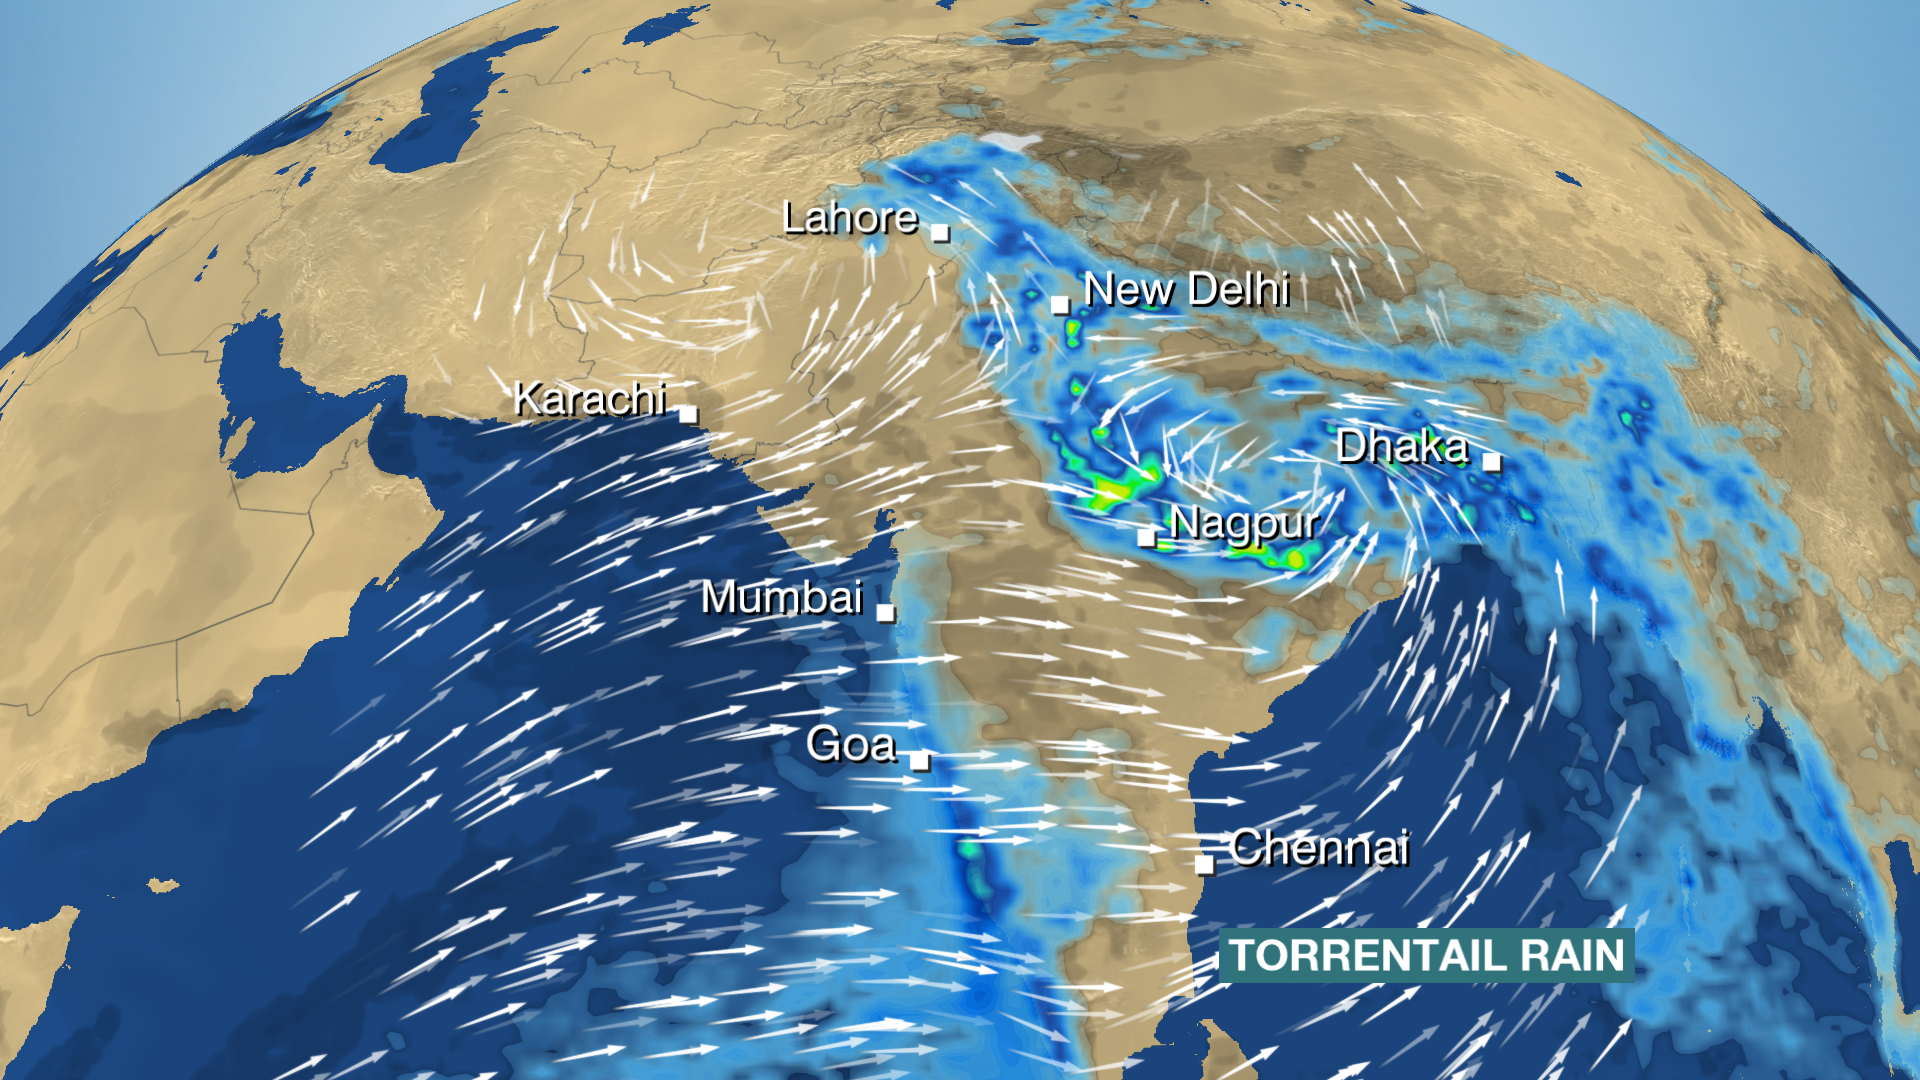
\includegraphics[height=0.5\textheight ,width=1\textwidth]{images/MD-sample.png}
			\caption{\footnotesize Schematic of a typical Monsoon Depression structure.}
			\label{fig:monsoon_dep}
		\end{figure}

		\vspace{-0.35cm}
		\begin{alertblock}{\small Importance}
			\scriptsize
			Contributes $\mathbf{50-60\%}$ of seasonal rainfall in Central and Northwest India, making its accurate simulation crucial for Indian agriculture and water resource management.
		\end{alertblock}
	\end{columns}
\end{frame}
%---------------------------------------------------------

%---------------------------------------------------------Slide 4
\setLayout{vertical}
\begin{frame}{Research Motivation}
	\footnotesize The accurate prediction of MD track, intensity, and associated heavy rainfall, particularly due to uncertainties in Land Surface Conditions (\textit{LSCs}).
	\vspace{0.4cm}

	\begin{columns}
		\column{0.58\textwidth}
		\textbf{\small Why study soil moisture-precipitation feedback?}
		\footnotesize
		\begin{itemize}
			\item \textbf{Hydrological Cycle:} Soil moisture influences evaporation and convection
			\item \textbf{Intensity Modulation:} May affect depression intensity and MD track
			\item \textbf{Predictability:} Potential improvement in forecasting
			\item \textbf{Climate Change:} Changing land-atmosphere interactions
		\end{itemize}

		\vspace{0.4cm}

		\begin{block}{\small The Feedback Loop}
			\centering
			\vspace{0.2cm}
			\footnotesize
			Soil Moisture $\rightleftharpoons$ Convection $\rightleftharpoons$ Precipitation
		\end{block}

		\column{0.45\textwidth}
		\vspace{-0.5cm}
		\begin{figure}
			\centering
			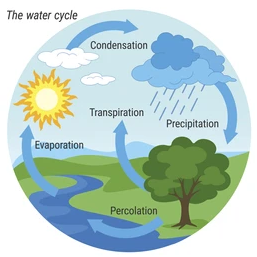
\includegraphics[width=0.7\textwidth]{images/water-cycle.png}
			\caption{\footnotesize Schematic of a Hydrological Cycle.}
			\label{fig:hyro-cycle}
		\end{figure}
	\end{columns}
\end{frame}
%---------------------------------------------------------

\subsection{Problem Statement}
%---------------------------------------------------------Slide 5
\setLayout{horizontal}
\begin{frame}{Problem Statement}
	\begin{columns}
		\column{0.39\textwidth}
		\vspace{0.4cm}
		\textbf{\small Research Questions:}
		\footnotesize
		\begin{enumerate}
			\item How does soil moisture initialization affect monsoon depression?
			\item What is the quantitative impact of soil moisture on precipitation rates?
			\item Does precipitation feedback alter soil moisture patterns?
			      % \item Investigate the hypothesized Land-Atmosphere (L-A) coupling where pre-existing or MD-induced soil moisture and precipitation anomalies impact the system's energy (Sensible/Latent Heat Fluxes).
			      % \item What are the dominant physical processes in this coupling?
		\end{enumerate}

		\column{0.61\textwidth}
		\vspace{-0.7cm}
		\begin{figure}
			\centering
			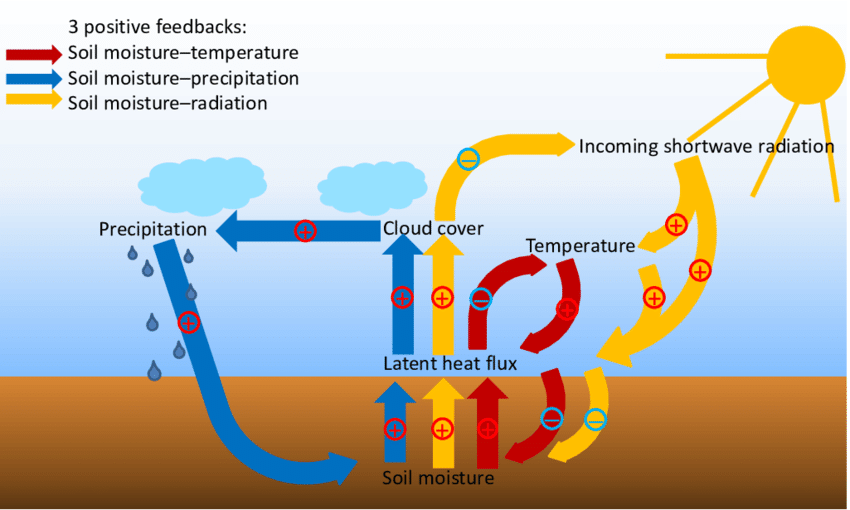
\includegraphics[width=\textwidth]{images/Soil-moisture-precipetation-feedback.png}
			\caption{\footnotesize Soil moisture-precipitation feedback}
			\label{fig:feedback}
		\end{figure}
	\end{columns}
\end{frame}
%---------------------------------------------------------

\subsection{Objectives}
%---------------------------------------------------------Slide 5
\setLayout{horizontal}
\begin{frame}{Objectives}
	% \textbf{\small Objectives:}
	\footnotesize
	Understanding the bidirectional relationship between soil moisture and precipitation in MD systems by:
	\begin{itemize}
		\item Objectively tracking MDs using a detection algorithm (based on MSLP and Wind speed).
		\item Quantify soil moisture-precipitation feedback mechanisms.
		\item Analyzing the \textit{radial structure} of key land surface and atmospheric variables (MSLP, Soil Moisture, Heat Fluxes) using \textit{Azimuthal Hovm\"oller Diagrams}.
		\item Quantifying the MD's \textit{translation speed} and its correlation with Land Surface Conditions (\textit{LSCs}).
		\item Analyze mesoscale dynamics of monsoon depression.
		      % \item Identify dominant physical processes in the coupling
	\end{itemize}
\end{frame}
%---------------------------------------------------------

\section{Data}
%---------------------------------------------------------Slide 7
\setLayout{mainpoint}
\begin{frame}{}
	\frametitle{DATA}
\end{frame}
%---------------------------------------------------------

%---------------------------------------------------------Slide 8
\setLayout{horizontal}
\begin{frame}{Dataset Overview}
	\begin{columns}
		\column{0.75\textwidth}
		\vspace{-0.6cm}
		\begin{block}{\small ERA5 (ECMWF Reanalysis version 5) Data}
			\footnotesize
			\begin{itemize}
				\item \textbf{Source:} ERA5 hourly data on single levels
				\item \textbf{Temporal Coverage:} July to September 2024
				\item \textbf{Spatial Domain:} 30°N-5°N, 70°E-100°E
				\item \textbf{Resolution:} 0.25° \(\times\) 0.25° (a grid cell of \(\approx\)27.75 km in latitude \(\times \approx\)24-28 km in longitude over the Indian subcontinent)
				\item \textbf{Frequency:} Hourly data
			\end{itemize}
		\end{block}

		\vspace{0.2cm}

		\begin{block}{\small Data Acquisition}
			\footnotesize
			\begin{itemize}
				\item \textbf{Available on:} European Union's Copernicus Climate Change Service (C3S),
				\item \textbf{Access via:} Copernicus Climate Data Store (CDS), offering hourly global atmospheric, land, and ocean data from 1940 to present.
				\item \textbf{Format:} Data stored in \texttt{NetCDF} format for analysis
			\end{itemize}
		\end{block}

		\column{0.25\textwidth}
		\vspace{-0.7cm}
		\begin{figure}
			\centering
			
\includegraphics[width=1\textwidth]{lib/logo/era5-logo.png}
			% \caption{\footnotesize ERA5 reanalysis data from ECMWF}
			\label{fig:era5}
		\end{figure}

		\vspace{0.2cm}

		\begin{figure}
			\centering
			
\includegraphics[width=1\textwidth]{lib/logo/Copernicus vecto def Europe's eyes on Earth.png}
			% \caption{\footnotesize ERA5 data provider }
			\label{fig:copernicus}
		\end{figure}

		\vspace{0.2cm}

		\begin{figure}
			\centering
			
\includegraphics[width=1\textwidth]{lib/logo/C3S–POS–LINE.png}
			% \caption{\footnotesize ERA5 data provider }
			\label{fig:cds}
		\end{figure}
	\end{columns}
\end{frame}
%---------------------------------------------------------

%---------------------------------------------------------Slide 9
\setLayout{horizontal}
\begin{frame}{Data Variables and Structure}
	\begin{columns}
		\column{0.47\textwidth}
		\begin{block}{\small \textbf{Instantaneous Variables}}
			\footnotesize
			\begin{itemize}
				\item \faIcon{thermometer-half}  2m temperature (\texttt{t2m})
				\item \faIcon{tachometer-alt} Mean sea level pressure (\texttt{msl})
				\item \faIcon{wind} 10m u-wind component (\texttt{u10})
				\item \faIcon{wind} 10m v-wind component (\texttt{v10})
				\item \faIcon{seedling} Soil temperature level 1 (\texttt{stl1})
				\item \faIcon{tint} Volumetric soil water layer 1 (\texttt{swvl1})
			\end{itemize}
		\end{block}

		\column{0.55\textwidth}
		\begin{block}{\small \textbf{Average Variables}}
			\footnotesize
			\begin{itemize}
				\item \faIcon{fire} Mean surface latent heat flux (\texttt{avg\_slhtf})
				\item \faIcon{sun} Mean surface sensible heat flux (\texttt{avg\_ishf})
			\end{itemize}
		\end{block}

		\vspace{0.8cm}

		\begin{block}{\small \textbf{Accumulated Variables}}
			\footnotesize
			\begin{itemize}
				\item \faIcon{cloud-rain} Total precipitation (\texttt{tp})
			\end{itemize}
		\end{block}
	\end{columns}
\end{frame}
%---------------------------------------------------------

%---------------------------------------------------------Slide 10
\setLayout{plain}
\begin{frame}{Study Domain and Temporal Coverage}
	\begin{columns}
		\vspace{-0.2cm}
		\column{0.45\textwidth}
		\begin{block}{\small \textbf{Spatial Domain}}
			\footnotesize
			\begin{itemize}
				\item \textbf{Latitude:} 30°N to 5°N
				\item \textbf{Longitude:} 70°E to 100°E
				\item \textbf{Area:} Covers Indian subcontinent and Bay of Bengal
				\item \textbf{Resolution:} 0.25° \(\times\) 0.25°
			\end{itemize}
		\end{block}

		\vspace{0.5cm}

		\begin{block}{\small \textbf{Temporal Coverage}}
			\footnotesize
			\begin{itemize}
				\item \textbf{Months} July-September 2024
				\item \textbf{Hourly Data:} Continuous temporal coverage
			\end{itemize}
		\end{block}

		\column{0.64\textwidth}
		\vspace{-1cm}
		\begin{figure}
			\centering
			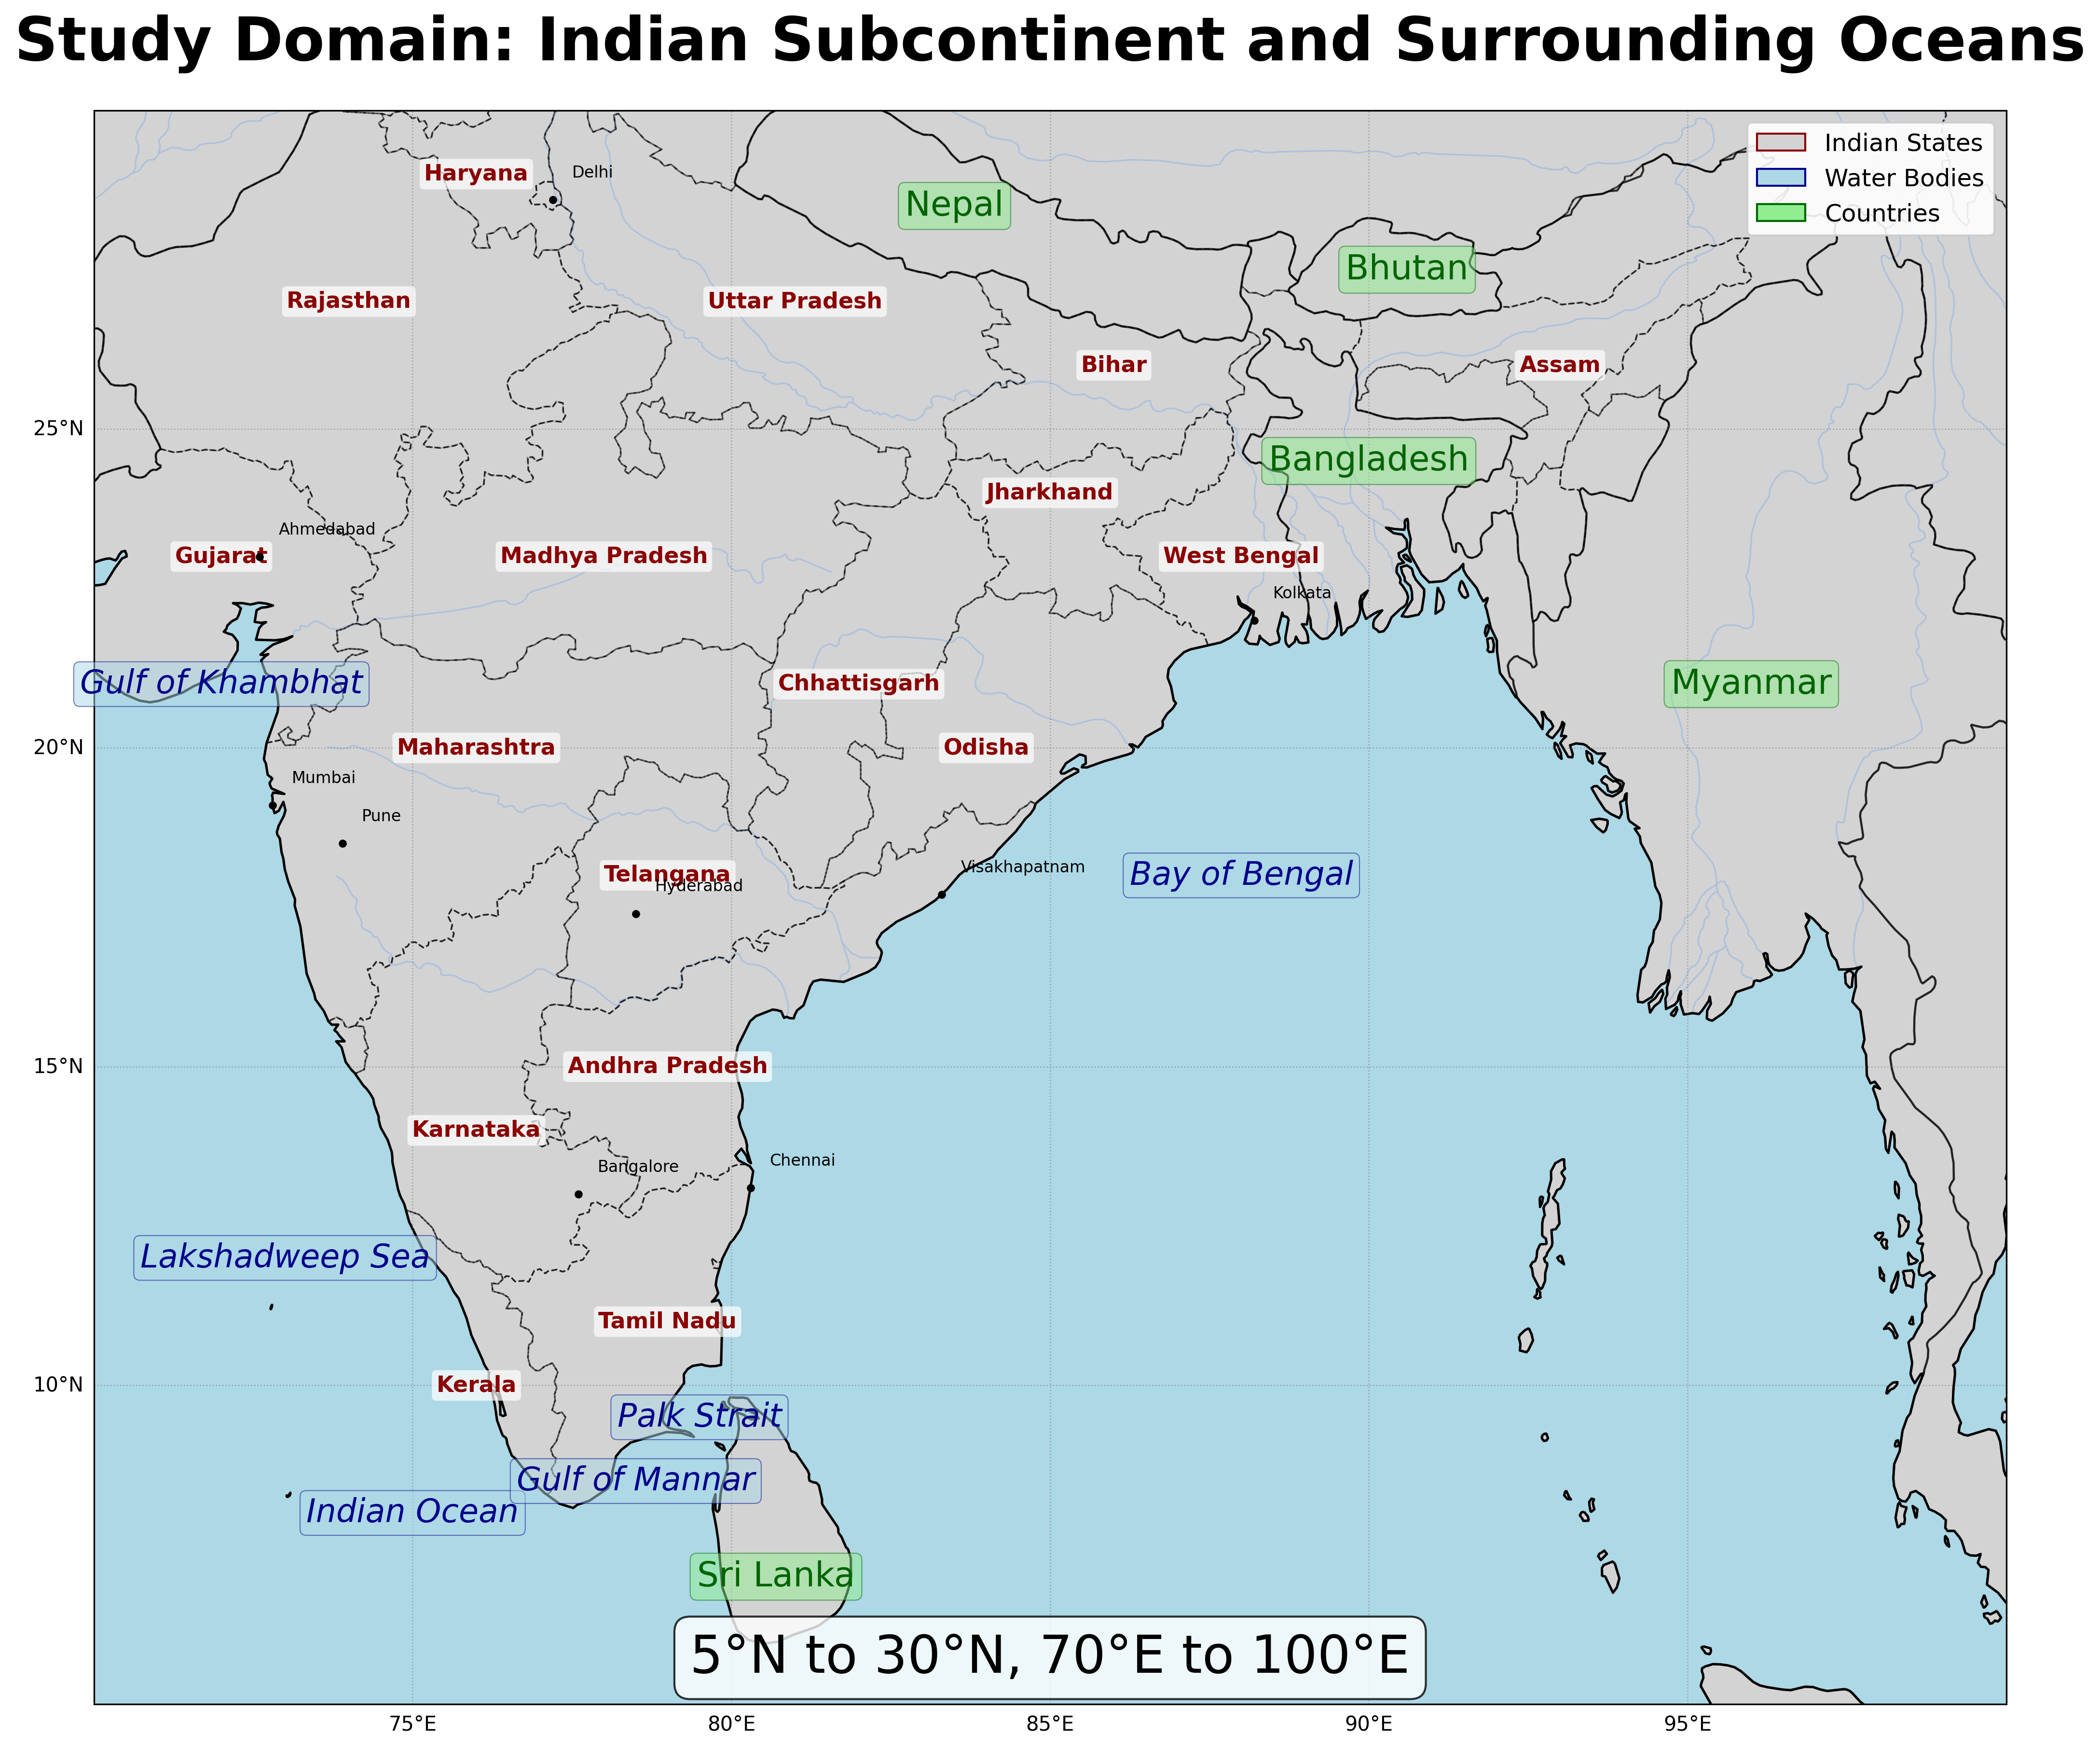
\includegraphics[width=1\textwidth]{images/study-domain.png}
			\caption{\footnotesize Study domain 30°N-5°N, 70°E-100°E}
			\label{fig:domain}
		\end{figure}
	\end{columns}
\end{frame}
%---------------------------------------------------------

%---------------------------------------------------------Slide 11
\setLayout{horizontal}
\begin{frame}{Variable Descriptions and Relevance}
	\vspace{-0.5cm}
	\begin{center}
		\begin{table}
			\centering
			\footnotesize
			\caption{Key ERA5 variables for monsoon depression analysis}
			\begin{tabular}{p{0.27\linewidth} p{0.14\linewidth} p{0.38\linewidth}}
				\toprule
				\rowcolor{MyBlue!20}
				\textbf{Variable}       & \textbf{Abbreviation} & \textbf{Relevance to MD Study}       \\
				\midrule
				2m temperature          & \texttt{t2m}          & Surface heating, convection trigger  \\
				Mean sea level pressure & \texttt{msl}          & Depression identification, intensity \\
				U/V wind components     & \texttt{u10, v10}     & Circulation pattern                  \\
				Soil temperature        & \texttt{stl1}         & Land surface energy balance          \\
				Soil moisture           & \texttt{swvl1}        & \textbf{Key feedback variable}       \\
				Total precipitation     & \texttt{tp}           & \textbf{Main response variable}      \\
				Latent heat flux        & \texttt{avg\_slhtf}   & Moisture transport, convection       \\
				Sensible heat flux      & \texttt{avg\_ishf}    & Surface heating, turbulence          \\
				\bottomrule
			\end{tabular}
			\label{tab:variables}
		\end{table}
	\end{center}
\end{frame}
%---------------------------------------------------------

\section{Methodology}
%---------------------------------------------------------Slide 12
\setLayout{mainpoint}
\begin{frame}{}
	\frametitle{METHODOLOGY}
\end{frame}
%---------------------------------------------------------

\subsection{MD Detection}
%---------------------------------------------------------Slide 13
\setLayout{vertical}
\begin{frame}{Monsoon Depression Detection and Tracking}
	\textbf{\small Detection Methodology}
	\footnotesize
	\begin{itemize}
		\item \textbf{Initial Filter:} Identify low-pressure systems ($\texttt{msl} < 1000 \text{ hPa}$) with cyclonic circulation ($8 \text{m/s} < \texttt{wind10} < 16 \text{ m/s}$)\footnotemark
		\item \textbf{Lifetime Filter:} Tracks must persist for a minimum \texttt{24} hours duration  to be classified as a valid MD.
		      % \item \textbf{Tracking Criteria:} Successive detections must satisfy time and distance thresholds:
		      %       \begin{itemize}
		      % 	      \item Max Distance: $300 \text{ km}$
		      % 	      \item Max Time Interval: $1 \text{ hour}$
		      %       \end{itemize}
	\end{itemize}

	\vspace{1.5cm}

	\begin{alertblock}{\small Output}
		\footnotesize
		Successfully detected 4 valid MD tracks during July-September 2024.
	\end{alertblock}

	\vspace{1cm}

	\hrule
	\footnotemark[1]{\tiny Adapted from the IMD criteria for Monsoon Depression identification. They uses $15 \text{knots} < 20 \text{knots}$ which is equivalent to $\sim 7.7 \text{m/s} < 13.5 \text{m/s}$ for wind speed thresholds. Source: \href{https://mausam.imd.gov.in/imd_latest/monsoonfaq.pdf}{IMD Monsoon FAQ}

		While ERA5 reanalysis dataset have surface wind speeds in the range of $8.5 < 16.5$ (m/s). }
\end{frame}
%---------------------------------------------------------

\subsection{Hovm\"oller Analysis}
%---------------------------------------------------------Slide 14 Hovm\"oller
\setLayout{vertical}
\begin{frame}{Hovm\"oller Analysis: A Shift to Relative Coordinates}
	\vspace{-0.2cm}
	\textbf{\small What are Hovm\"oller Plots?}
	\footnotesize
	\begin{itemize}
		\item Visual tool for analyzing wave and storm propagation.
		\item \textbf{Classical Definition:} Plots a variable's intensity over one $\textbf{fixed spatial dimension}$ (Longitude or Latitude) against $\textbf{time}$. (Shows movement across a region).
	\end{itemize}

	\vspace{0.5cm}

	\textbf{\small Azimuthal Hovmöller}
	\footnotesize
	\begin{itemize}
		\item Used a relative coordinate system to track the MD's internal structure as it propagate.
		\item The X-axis (spatial) is the $\textbf{Radius from the storm center}$ (km).
		\item The Y-axis (temporal) remains $\textbf{Time}$ along the MD track.
	\end{itemize}

	\vspace{-1cm}
	\begin{alertblock}{\small Why Azimuthal?}
		\footnotesize
		\textbf{Advantage:} It isolates the evolution of the storm's $\textbf{radial structure}$ (e.g., core deepening, widening of rainfall) from its $\textbf{translational movement}$ across the map.
	\end{alertblock}
\end{frame}
%---------------------------------------------------------

\subsection{Azimuthal Averaging}
%---------------------------------------------------------Slide 15: Azimuthal Averaging
\setLayout{horizontal}
\begin{frame}{Azimuthal Averaging}
	\vspace{-0.2cm}
	\footnotesize
	\begin{enumerate}
		\item \textbf{Center Identification:} The MD center (minimum $\texttt{msl}$ location) is determined at hourly time step from the tracking data.
		\item \textbf{Radial Grid Definition:} Concentric rings are defined around the center, typically starting at increments of $25 \text{ km}$ and extending up to $350 \text{ km}$ radius.
		\item \textbf{Nearest Grid Point Search:} For each ring (annulus), find all ERA5 grid points that fall within that specific radial distance bin.
		\item \textbf{Averaging:} The mean value of the variable ($\texttt{swvl1}$, $\texttt{tp}$, $\texttt{msl}$, $\texttt{avg\_ishf}$, $\texttt{avg\_slhf}$, $\texttt{t2m}$, $\texttt{wind10m}$) is calculated across all identified grid points in that ring.
	\end{enumerate}

	\vspace{-1cm}

	\footnotesize
	\begin{alertblock}{\small Resulting Hovm\"oller Array}
		\begin{itemize}
			\item This process transforms the 3D data (Lat $\times$ Lon $\times$ Time) into a 2D array ($\textbf{Radius} \times \textbf{Time}$).
		\end{itemize}
	\end{alertblock}
\end{frame}

%---------------------------------------------------------Slide 16: Azimuthal Averaging
\setLayout{plain}
\begin{frame}{Azimuthal Averaging}
	\begin{columns}
		\column{0.62\textwidth}
		\vspace{-1.1cm}
		\begin{figure}
			\centering
			\begin{tikzpicture}[
					scale=0.5,
					% Define styles
					grid/.style={circle, inner sep=1.5pt, draw=black, very thin},
					ring/.style={draw=MyBlue!70, dashed, thin},
					center/.style={fill=MyBlue, circle, inner sep=2pt, draw=black},
					mdlabel/.style={text=MyBlue!80, font=\tiny}
				]

				% Grid background
				\draw[step=1cm, draw=gray!40, very thin] (-6.3,-6.4) grid (6.3,6.4);
				\node[font=\footnotesize, fill=white, inner sep=1pt] at (4, 5.5) {ERA5 Grid ($0.25^\circ \times 0.25^\circ$)};
				\node[font=\footnotesize, fill=white, inner sep=1pt] at (-5, 5.5) {At time $t$};

				% MD Center
				\coordinate (C) at (0,0);
				\node[center, label={[mdlabel]below:MD Center}] (MD) at (C) {};

				% Concentric circles
				\draw[ring] (C) circle (1.0);
				\draw[ring] (C) circle (2.0);
				\draw[ring, MyBlue!90, thick] (C) circle (3.0);
				\draw[ring] (C) circle (4.0);
				\draw[ring] (C) circle (6.0);

				% ERA5 GRID POINTS
				% \foreach \x in {-6,-5,...,6}{
				% 		\foreach \y in {-6,-5,...,6}{
				% 				\node[grid, fill=blue!20] at (\x,\y) {};
				% 			}
				% 	}

				% RADIAL BIN POINTS
				\node[grid, fill=red!70] (P1) at (2.55, -1.55) {};
				\node[grid, fill=red!70] (P2) at (-1.6, 3.65) {};
				\node[grid, fill=red!70] (P3) at (-2.55, -1.55) {};
				\node[grid, fill=red!70] (P4) at (3.6, 1.6) {};
				\node[grid, fill=red!70] (P5) at (1.5, 2.5) {};
				\node[grid, fill=red!70] (P6) at (-2.6, 1.5) {};

				% Sample bin points near 75 km radius
				\node[grid, fill=blue!50] (PB1) at (3, -1) {};
				\node[grid, fill=blue!50] (PB2) at (3, -2) {};
				\node[grid, fill=blue!50] (PB3) at (2, -2) {};
				\node[grid, fill=blue!50] (PB4) at (2, -1) {};

				% Distance labels
				% \draw[-, very thick, black!70] (0, 0) -- node[above, font=\tiny] {$25 \text{ km}$} (1, 0);
				\draw[-, very thick, black!70] (0, 0) -- node[font=\tiny] {$350 \text{ km}$} (-4.24, 4.24);
				\draw[<->, very thick, black!75] (-2, 0) -- node[above, font=\tiny] {$25 \text{ km}$} (-3, 0);

				% Info box
				\node[draw=black!40, thick, rounded corners, align=left, fill=red!5, text=black, anchor=west]
				at (-0.6, -4.6) (AveragingBox)
				{\tiny \textbf{Azimuthal Average:}\\
					\tiny $\overline{V}(R) = \frac{1}{N}\sum_{i=1}^{N} V_i$\\
					\tiny $\textbf{N}$: No. of grid points in bin
					\vspace{-0.3cm}\\
					\tiny $\textbf{R}$: Radial bin (at $75$ to $100\text{ km}$)
				};

				% Arrow
				\draw[->, very thick, red!80, shorten >= 3pt, shorten <= 3pt] (AveragingBox.north) -- (P1);

				% legend
				\node[draw=black!40, rounded corners, fill=gray!10, anchor=north west, inner sep=2pt]
				at (4, 5) (legend) {
					\begin{tikzpicture}[scale=1]
						% ERA5 GRID POINTS
						\node[grid, fill=blue!50] at (0,0) {};
						\node[anchor=west, font=\tiny] at (0.2,-0.05) {ERA5 Grid Points};
						% RADIAL BIN POINTS
						\node[grid, fill=red!70] at (0,-0.35) {};
						\node[anchor=west, font=\tiny] at (0.2,-0.40) {Points in Bin};
					\end{tikzpicture}
				};

			\end{tikzpicture}
			\caption{\footnotesize Schematic of the Azimuthal Averaging method applied to the ERA5 grid.}
		\end{figure}

		\column{0.56\textwidth}
		\textbf{\small Azimuthal Averaging Procedure}
		\scriptsize
		\begin{itemize}
			\setlength\itemsep{0.5pt}
			\item \textbf{Center:} The MD center is defined at each time step of 1 hour using the location of the minimum MSLP.
			\item \textbf{Radial Bins:} Radial distances are sampled every $25$ km up to $350$ km: \(R = \{0, 25, 50, \dots, 350\} \text{ km}\)
			\item \textbf{Adaptive Ring Thickness:} Points are selected within a ring of half-width:  \(dR = \max(10\text{ km},\, 0.15R),\)
			\item \textbf{Sampling:} For each radius $R$, all ERA5 grid points that lie inside
			      $(R - dR)$ to $(R + dR)$ are extracted.
			\item \textbf{Azimuthal Mean:} The average of all $N$ points in the ring is computed: \(\overline{V}(R) = \frac{1}{N}\sum_{i=1}^{N} V_i\).
		\end{itemize}

		\vspace{0.5cm}

		\begin{alertblock}{\small Output → Hovm\"oller Diagram}
			\scriptsize
			A 2D field: \(\textbf{Radius (X)} \times \textbf{Time (Y)} \) for each variable.

			The evolution of the radial structure with time \(\texttt{t}\) is visualized using a Hovm\"oller plot.
		\end{alertblock}
	\end{columns}
\end{frame}
%---------------------------------------------------------

\section{Methodology: Translation Speed Analysis}
%---------------------------------------------------------Slide 17
\setLayout{vertical}
\begin{frame}{MD Translation Speed Analysis}
	\vspace{-0.4cm}
	\footnotesize
	\begin{itemize}
		\item \textbf{Speed Calculation (Translation Speed):} The magnitude of the movement of the disturbance center between consecutive timesteps.
		      \begin{center}
			      $$\text{Translation Speed} = \frac{\textbf{Geodesic Distance} (t \to t+\Delta t)}{\Delta t} \quad (\text{km/hr})$$
		      \end{center}
		\item \textbf{Temporal Resolution ($\Delta t$):} The calculation is performed over the $\mathbf{1\text{-hour}}$ data interval ($\Delta t = 1\text{ hr}$).
		\item \textbf{Track Stage Classification:} Tracks are classified into distinct stages (e.g., Genesis, Intensification, Decay) based on specific meteorological criteria for detailed speed analysis.
	\end{itemize}

	% \begin{itemize}
	% 	\item \textbf{Geodesic Distance ($\textbf{d}$):}
	% 	      \begin{enumerate}
	% 		      \item The \textbf{shortest path} between two points on the surface of a curved space (e.g., the Earth).
	% 		      \item It follows the arc of the **Great Circle**—a circle on the sphere whose center is the center of the sphere itself.
	% 		      \item \textbf{Justification:} Using a planar (flat-map) distance formula (like the Euclidean distance) leads to **significant errors** for moving systems, especially at high latitudes, due to Earth's spherical nature.
	% 	      \end{enumerate}
	%
	% 	\item \textbf{Distance Method: The Haversine Formula}
	% 	      \begin{enumerate}
	% 		      \item This specific formula is a **robust mathematical tool** for calculating the Great Circle distance given two points (latitude $\phi$, longitude $\lambda$) on a sphere.
	% 		      \item The implementation from the $\texttt{geopy}$ library is used: $\texttt{geopy.distance.geodesic}$ (which internally uses the Haversine method for Earth-like models).
	% 		      \item \textbf{The Haversine Function ($\text{hav}$):}
	% 		            \begin{center}
	% 			            $$\text{hav}(\theta) = \sin^2\left(\frac{\theta}{2}\right)$$
	% 		            \end{center}
	% 		      \item **The Formula:** It relates the difference in latitude and longitude ($\Delta\phi, \Delta\lambda$) to the central angle ($\Delta\sigma$) between the two points, ultimately yielding the distance $\textbf{d}$:
	% 		            \begin{center}
	% 			            $$\mathbf{d} = 2R \cdot \arcsin\left(\sqrt{\text{hav}(\phi_2-\phi_1) + \cos(\phi_1)\cos(\phi_2)\text{hav}(\lambda_2-\lambda_1)}\right)$$
	% 		            \end{center}
	% 		            \vspace{-0.2cm}
	% 		            \emph{Where $R$ is the radius of the Earth.}
	% 	      \end{enumerate}
	% \end{itemize}

	\vspace{0.4cm}

	\begin{alertblock}{\small Goal: Statistical Quantification}
		Quantify how land-surface interaction (e.g., dry vs. wet soil) statistically correlates with the depression's translation speed.
		\vspace{0.1cm}
		\begin{itemize}
			\item [\(\checkmark\)] Statistical significance of speed differences is tested using the $\textbf{non-parametric Mann-Whitney U Test}$ (imported from $\texttt{scipy.stats}$).
		\end{itemize}
	\end{alertblock}
\end{frame}
%---------------------------------------------------------

\section{Results: Dynamics and Structure}
%---------------------------------------------------------Slide 18
\setLayout{mainpoint}
\begin{frame}{}
	\frametitle{RESULTS}
\end{frame}
%---------------------------------------------------------

%---------------------------------------------------------Slide 19 all track
\setLayout{plain}
\begin{frame}{Results: MD Tracks and comparison with IMD Report}
	\begin{columns}[c]
		\column{0.48\textwidth}
		\vspace{-0.5cm}
		\begin{figure}
			\centering
			\includegraphics[width=0.96\textwidth]{../output/MD-track.png}
			\caption{\scriptsize All detected MD tracks from \\ July to September 2024}
		\end{figure}

		\column{0.52\textwidth}
		\vspace{-0.3cm}
		\begin{figure}
			\centering
			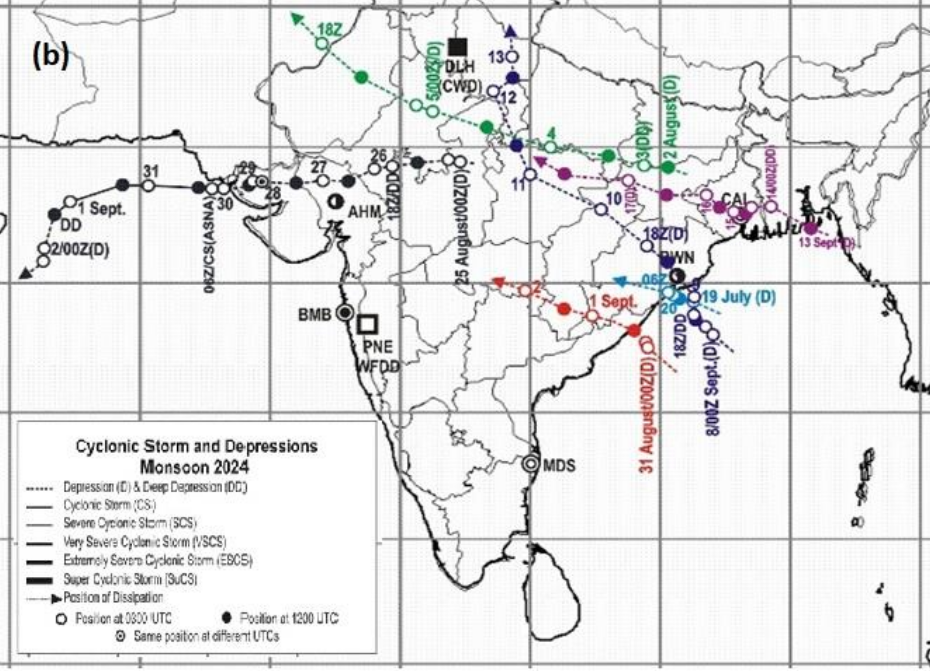
\includegraphics[width=0.99\textwidth]{images/IMD-report.png}
			\caption{\scriptsize IMD monsoon tracks report \\ for 2024\footnotemark[1]}
		\end{figure}
	\end{columns}

	\vspace{0.3cm}
	\hrule
	\footnotemark[1]{\tiny India Meteorological Department (IMD) 2024 Monsoon Report, \\Source: \href{https://mausam.imd.gov.in/responsive/monsooninformation.pdf}{\url{https://mausam.imd.gov.in/responsive/monsooninformation.php}}}
\end{frame}
%---------------------------------------------------------

%---------------------------------------------------------Slide 20 track 1
\setLayout{horizontal}
\begin{frame}{Results: MD Track and Evolution (Track 1)}
	\begin{columns}
		\column{0.35\textwidth}
		\vspace{-0.5cm}
		\begin{block}{\small Track Summary (Track 1)}
			\footnotesize
			\begin{itemize}
				\item \textbf{Time Span:} 2024-07-18 to 2024-07-21
				\item \textbf{Duration:} $\approx$ 66 hours (2 days  18 hrs)
			\end{itemize}
		\end{block}

		\vspace{2cm}
		\begin{alertblock}{\small Note}
			\footnotesize
			Tracking confirms the traditional BOB-to-landfall trajectory common for monsoon depressions.
		\end{alertblock}

		\column{0.65\textwidth}
		\vspace{-1.10cm}
		\begin{figure}
			\centering
			\includegraphics[width=\textwidth]{../output/track_1/MD-track-1-cropped.png}
			% \caption{}
		\end{figure}
	\end{columns}
\end{frame}
%---------------------------------------------------------

% Hovmoller plots
%---------------------------------------------------------Slide 21
\setLayout{plain}
\begin{frame}{Soil Water Content Hovm\"oller for Track 1}
	\begin{columns}
		\column{0.7\textwidth}
		\vspace{-1.2cm}
		\begin{figure}
			\centering
			\includegraphics[width=\textwidth]{../output/track_1/hovmoller/hov_swvl1.png}
			\caption{\footnotesize Soil Moisture Hovm\"oller plot for Track 1}
		\end{figure}

		\column{0.3\textwidth}
		\begin{block}{\small Analysis}
			\footnotesize
			\begin{itemize}
				\item \textbf{Soil Moisture:} Significant increase in $\texttt{swvl1}$ (wetting) starts outside the core ($>100 \text{ km}$ radius) and persists long after the pressure minimum passes, showing the $\textbf{precipitation feedback}$.
			\end{itemize}
		\end{block}
	\end{columns}
\end{frame}
%---------------------------------------------------------

%---------------------------------------------------------Slide 22
\setLayout{plain}
\begin{frame}{Total Precipitation Hovm\"oller for Track 1}
	\begin{columns}
		\column{0.72\textwidth}
		\vspace{-1.2cm}
		\begin{figure}
			\centering
			\includegraphics[width=\textwidth]{../output/track_1/hovmoller/hov_tp.png}
			\caption{\footnotesize Total Precipitation Hovm\"oller plot for Track 1}
		\end{figure}

		\column{0.3\textwidth}
		\vspace{-1cm}
		\begin{block}{\small Analysis}
			\footnotesize
			\begin{itemize}
				\item Intense rainfall begins in outer radii ($>100$ km) before the depression arrives.
				\item Strongest precipitation aligns with the pressure minimum and persists behind it, matching the observed soil-moisture increase.
			\end{itemize}
		\end{block}

		\vspace{0.2cm}

		\begin{alertblock}{\footnotesize Precipitation Intensity Note}
			\tiny
			\begin{itemize}
				\item Values represent \textbf{azimuthal averages} over 360\(^\circ\) rings - heavy rainfall in narrow bands gets diluted.
				\item Precipitation in MDs is often asymmetric (concentrated in sectors), not uniform around the center.
				\item Peak intensities would be higher in localized rainbands. \\
			\end{itemize}
		\end{alertblock}
	\end{columns}
\end{frame}
%---------------------------------------------------------

%---------------------------------------------------------Slide 23
\setLayout{plain}
\begin{frame}{Surface Latent Heat Flux Hovm\"oller for Track 1}
	\begin{columns}
		\column{0.72\textwidth}
		\vspace{-1.2cm}
		\begin{figure}
			\centering
			\includegraphics[width=\textwidth]{../output/track_1/hovmoller/hov_avg_ishf.png}
			\caption{\footnotesize Surface Latent Heat Flux Hovm\"oller plot for Track 1}
		\end{figure}

		\column{0.3\textwidth}
		\vspace{-0.8cm}
		\begin{block}{\small Analysis}
			\footnotesize
			\begin{itemize}
				\item Initially shows negative values (flux from atmosphere to surface) indicating condensation/rainfall as the system approaches.
				\item Positive values after passage indicate enhanced evaporation from the surface, showing moisture recovery.
				\item The sign reversal confirms the precipitation-evaporation feedback cycle.
			\end{itemize}
		\end{block}
	\end{columns}
\end{frame}
%---------------------------------------------------------

%---------------------------------------------------------Slide 24
\setLayout{plain}
\begin{frame}{Surface Sensible Heat Flux Hovm\"oller for Track 1}
	\begin{columns}
		\column{0.72\textwidth}
		\vspace{-1.2cm}
		\begin{figure}
			\centering
			\includegraphics[width=\textwidth]{../output/track_1/hovmoller/hov_avg_slhtf.png}
			\caption{\footnotesize Surface Sensible Heat Flux Hovm\"oller plot for Track 1}
		\end{figure}

		\column{0.3\textwidth}
		\vspace{-0.8cm}
		\begin{block}{\small Analysis}
			\footnotesize
			\begin{itemize}
				\item Negative values near the core indicate cooling from rainfall and cloud cover (heat flux from atmosphere to surface).
				\item Positive values in outer radii and post-depression show surface heating (heat flux from surface to atmosphere).
				\item The transition from negative to positive values marks the shift from convective cooling to surface reheating.
			\end{itemize}
		\end{block}
	\end{columns}
\end{frame}
%---------------------------------------------------------

%---------------------------------------------------------Slide 25
\setLayout{plain}
\begin{frame}{10 Metre Wind Speed Hovm\"oller for Track 1}
	\begin{columns}
		\column{0.72\textwidth}
		\vspace{-1.2cm}
		\begin{figure}
			\centering
			\includegraphics[width=\textwidth]{../output/track_1/hovmoller/hov_wind10.png}
			\caption{\footnotesize 10m wind speed Hovm\"oller plot for Track 1}
		\end{figure}

		\column{0.3\textwidth}
		\vspace{-0.8cm}
		\begin{block}{\small Analysis}
			\footnotesize
			\begin{itemize}
				\item \textbf{Wind Field:} Maximum wind speeds occur at more than $50$ km radius.
				\item Wind speeds are lower within the core ($<50$ km), consistent with the low-pressure center.
				\item Wind speed decreases after the depression passes, indicating weakening circulation.
			\end{itemize}
		\end{block}
	\end{columns}
\end{frame}
%---------------------------------------------------------

%---------------------------------------------------------Slide 26
\setLayout{plain}
\begin{frame}{2 Metre Air Temperature Hovm\"oller for Track 1}
	\begin{columns}
		\column{0.72\textwidth}
		\vspace{-1.2cm}
		\begin{figure}
			\centering
			\includegraphics[width=\textwidth]{../output/track_1/hovmoller/hov_t2m.png}
			\caption{\footnotesize Air temperature at 2m above ground Hovm\"oller plot for Track 1}
		\end{figure}

		\column{0.3\textwidth}
		\vspace{-0.8cm}
		\begin{block}{\small Analysis}
			\footnotesize
			\begin{itemize}
				\item A cooling trend is observed as the depression approaches, especially within $100$ km radius, due to cloud cover and rainfall.
				\item Post-depression, temperatures gradually recover as skies clear and solar heating resumes.
				\item Core is warmer relative to surrounding areas, likely due to subsidence warming effects.
			\end{itemize}
		\end{block}
	\end{columns}
\end{frame}
%---------------------------------------------------------

%---------------------------------------------------------Slide 27
\setLayout{plain}
\begin{frame}{Mean Sea Level Hovm\"oller for Track 1}
	\begin{columns}
		\column{0.72\textwidth}
		\vspace{-1.2cm}
		\begin{figure}
			\centering
			\includegraphics[width=\textwidth]{../output/track_1/hovmoller/hov_msl.png}
			\caption{\footnotesize MSL Hovm\"oller plot for Track 1}
		\end{figure}

		\column{0.3\textwidth}
		\begin{block}{\small Analysis}
			\footnotesize
			\begin{itemize}
				\item The pressure minimum (depression core) is concentrated within the $50 \text{ km}$ radius.
			\end{itemize}
		\end{block}
	\end{columns}
\end{frame}
%---------------------------------------------------------

%---------------------------------------------------------Slide 28
\setLayout{plain}
\begin{frame}{Translation Speed Analysis for Track 1}
	\begin{columns}
		\column{0.72\textwidth}
		\vspace{-1cm}
		\begin{figure}
			\centering
			\includegraphics[width=\textwidth]{../output/track_1/windspeed/track_1_speed_timeseries.png}
			\caption{\footnotesize Translation Speed Analysis plot for Track 1}
		\end{figure}

		\column{0.3\textwidth}
		\begin{block}{\small Analysis}
			\footnotesize
			\begin{itemize}
				\item \textbf{Movement Speed:} The system accelerates slightly during intensification, then slows as it approaches landfall.
				\item Speed fluctuations reflect interaction with monsoon flow and terrain.
			\end{itemize}
		\end{block}
	\end{columns}
\end{frame}
%---------------------------------------------------------

%---------------------------------------------------------Slide 29 track 3
\setLayout{horizontal}
\begin{frame}{Results: MD Track and Evolution (Track 2)}
	\begin{columns}
		\column{0.35\textwidth}
		\vspace{-0.5cm}
		\begin{block}{\small Track Summary (Track 2)}
			\footnotesize
			\begin{itemize}
				\item \textbf{Time Span:} 2024-08-30 to 2024-09-01
				\item \textbf{Duration:} $\approx$ 56 hours (2days  8hrs)
			\end{itemize}
		\end{block}

		% \vspace{0.2cm}
		% \begin{alertblock}{\small Note}
		% 	\footnotesize
		% 	Tracking confirms the traditional BOB-to-landfall trajectory common for monsoon depressions.
		% \end{alertblock}

		\column{0.65\textwidth}
		\vspace{-1.10cm}
		\begin{figure}
			\centering
			\includegraphics[width=\textwidth]{../output/track_3/MD-track-3-cropped.png}
			% \caption{\footnotesize }
		\end{figure}
	\end{columns}
\end{frame}

%---------------------------------------------------------Slide 30
\setLayout{plain}
\begin{frame}{Soil Water Content Hovm\"oller for Track 2}
	\begin{columns}
		\column{0.7\textwidth}
		\vspace{-1.2cm}
		\begin{figure}
			\centering
			\includegraphics[width=\textwidth]{../output/track_3/hovmoller/hov_swvl1.png}
			\caption{\footnotesize Soil Moisture Hovm\"oller plot for Track 2}
		\end{figure}

		\column{0.3\textwidth}
		\begin{block}{\small Analysis}
			\footnotesize
			\begin{itemize}
				\item Strong moistening begins outside the core, mirroring Track 1 but with a shorter recovery timescale.
				\item Indicates sustained rainfall even after the center has passed.
			\end{itemize}
		\end{block}
	\end{columns}
\end{frame}
%---------------------------------------------------------

%---------------------------------------------------------Slide 31
\setLayout{plain}
\begin{frame}{Total Precipitation Hovm\"oller for Track 2}
	\begin{columns}
		\column{0.72\textwidth}
		\vspace{-1.2cm}
		\begin{figure}
			\centering
			\includegraphics[width=\textwidth]{../output/track_3/hovmoller/hov_tp.png}
			\caption{\footnotesize Total Precipitation Hovm\"oller plot for Track 2}
		\end{figure}

		\column{0.3\textwidth}
		\begin{block}{\small Analysis}
			\footnotesize
			\begin{itemize}
				\item Outer-radius rainfall precedes core passage; a broad rain shield follows the MD.
				\item Heaviest rainfall coincides with the minimum pressure radius less than $100$ km.
			\end{itemize}
		\end{block}
	\end{columns}
\end{frame}
%---------------------------------------------------------

%---------------------------------------------------------Slide 32
\setLayout{plain}
\begin{frame}{Surface Latent Heat Flux Hovm\"oller for Track 2}
	\begin{columns}
		\column{0.72\textwidth}
		\vspace{-1.2cm}
		\begin{figure}
			\centering
			\includegraphics[width=\textwidth]{../output/track_3/hovmoller/hov_avg_ishf.png}
			\caption{\footnotesize Surface Latent Heat Flux Hovm\"oller plot for Track 2}
		\end{figure}

		\column{0.3\textwidth}
		% \vspace{-0.8cm}
		\begin{block}{\small Analysis}
			\footnotesize
			\begin{itemize}
				\item Transition from negative (condensation/rain) to positive (evaporation) values.
				\item Enhanced evaporation ahead of MD provides moisture supply.
				\item Cloud cover near core suppresses surface evaporation.
			\end{itemize}
		\end{block}
	\end{columns}
\end{frame}
%---------------------------------------------------------

%---------------------------------------------------------Slide 33
\setLayout{plain}
\begin{frame}{Surface Sensible Heat Flux Hovm\"oller for Track 2}
	\begin{columns}
		\column{0.72\textwidth}
		\vspace{-1.2cm}
		\begin{figure}
			\centering
			\includegraphics[width=\textwidth]{../output/track_3/hovmoller/hov_avg_slhtf.png}
			\caption{\footnotesize Surface Sensible Heat Flux Hovm\"oller plot for Track 2}
		\end{figure}

		\column{0.3\textwidth}
		% \vspace{-0.8cm}
		\begin{block}{\small Analysis}
			\footnotesize
			\begin{itemize}
				\item Negative values in rainfall core show surface cooling.
				\item Positive values post-depression indicate surface reheating.
			\end{itemize}
		\end{block}

		\vspace{0.2cm}
		\begin{alertblock}{\footnotesize Track 2 Specific}
			\tiny
			\begin{itemize}
				\item Weaker cooling signal suggests less intense rainfall compared to Track 1.
				\item \textbf{Weaker heat flux signals:} Compared to Track 1, indicating less intense land-atmosphere coupling.
				\item \textbf{Shorter duration:} 56 hours vs. 66 hours for Track 1.
				\item \textbf{Later season:} August-September system may have different surface conditions.
			\end{itemize}
		\end{alertblock}
	\end{columns}
\end{frame}
%---------------------------------------------------------

%---------------------------------------------------------Slide 34
\setLayout{plain}
\begin{frame}{10 Metre Wind Speed Hovm\"oller for Track 2}
	\begin{columns}
		\column{0.72\textwidth}
		\vspace{-1.2cm}
		\begin{figure}
			\centering
			\includegraphics[width=\textwidth]{../output/track_3/hovmoller/hov_wind10.png}
			\caption{\footnotesize 10m wind speed Hovm\"oller plot for Track 2}
		\end{figure}

		\column{0.3\textwidth}
		\vspace{-0.7cm}
		\begin{block}{\small Analysis}
			\footnotesize
			\begin{itemize}
				\item Wind maxima develop just outside the core, consistent with a strong pressure gradient.
				\item \textbf{Wind Field:} Maximum wind speeds occur at more than $125$ km radius.
				\item Wind speeds are lower within the core ($<75$ km), consistent with the low-pressure center.
				\item Wind speed decreases after the depression passes, indicating weakening circulation and resistant propagation over land.
			\end{itemize}
		\end{block}
	\end{columns}
\end{frame}
%---------------------------------------------------------

%---------------------------------------------------------Slide 35
\setLayout{plain}
\begin{frame}{2 Metre Air Temperature Hovm\"oller for Track 2}
	\begin{columns}
		\column{0.72\textwidth}
		\vspace{-1.2cm}
		\begin{figure}
			\centering
			\includegraphics[width=\textwidth]{../output/track_3/hovmoller/hov_t2m.png}
			\caption{\footnotesize Air temperature at 2m above ground Hovm\"oller plot for Track 2}
		\end{figure}

		\column{0.3\textwidth}
		\begin{block}{\small Analysis}
			\footnotesize
			\begin{itemize}
				\item Outer-radius warming hints at pre-storm mixing.
				\item Warm-core structure is evident, with higher temperatures near the core due to latent heat release and subsidence.
				\item Post-depression cooling is observed as the system moves inland, consistent with cloud.
			\end{itemize}
		\end{block}
	\end{columns}
\end{frame}
%---------------------------------------------------------

%---------------------------------------------------------Slide 36
\setLayout{plain}
\begin{frame}{Mean Sea Level Hovm\"oller for Track 2}
	\begin{columns}
		\column{0.72\textwidth}
		\vspace{-1.2cm}
		\begin{figure}
			\centering
			\includegraphics[width=\textwidth]{../output/track_3/hovmoller/hov_msl.png}
			\caption{\footnotesize MSL Hovm\"oller plot for Track 2}
		\end{figure}

		\column{0.3\textwidth}
		\begin{block}{\small Analysis}
			\footnotesize
			\begin{itemize}
				\item The pressure minimum (depression core) is concentrated mostly within the $75 \text{ km}$ radius.
			\end{itemize}
		\end{block}
	\end{columns}
\end{frame}
%---------------------------------------------------------

%---------------------------------------------------------Slide 37
\setLayout{plain}
\begin{frame}{Translation Speed Analysis for Track 2}
	\begin{columns}
		\column{0.72\textwidth}
		\vspace{-1cm}
		\begin{figure}
			\centering
			\includegraphics[width=\textwidth]{../output/track_3/windspeed/track_3_speed_timeseries.png}
			\caption{\footnotesize Translation Speed Analysis plot for Track 2}
		\end{figure}

		\column{0.3\textwidth}
		\begin{block}{\small Analysis}
			\footnotesize
			\begin{itemize}
				\item Steady slow translation supports prolonged rainfall over the same region.
			\end{itemize}
		\end{block}
	\end{columns}
\end{frame}
%---------------------------------------------------------

%---------------------------------------------------------Slide 38 track 4
\setLayout{horizontal}
\begin{frame}{Results: MD Track and Evolution (Track 3)}
	\begin{columns}
		\column{0.34\textwidth}
		\vspace{-0.5cm}
		\begin{block}{\small Track Summary (Track 3)}
			\footnotesize
			\begin{itemize}
				\item \textbf{Time Span:} 2024-09-09 to 2024-09-10
				\item \textbf{Duration:} $\approx$ 84 hours (3days  12hrs)
			\end{itemize}
		\end{block}

		\column{0.68\textwidth}
		\vspace{-1.2cm}
		\begin{figure}
			\centering
			\includegraphics[width=0.95\textwidth]{../output/track_4/MD-track-4-cropped.png}
			% \caption{\footnotesize }
		\end{figure}
	\end{columns}
\end{frame}
%---------------------------------------------------------

%---------------------------------------------------------Slide 39
\setLayout{plain}
\begin{frame}{Soil Water Content Hovm\"oller for Track 3}
	\begin{columns}
		\column{0.7\textwidth}
		\vspace{-1.2cm}
		\begin{figure}
			\centering
			\includegraphics[width=\textwidth]{../output/track_4/hovmoller/hov_swvl1.png}
			\caption{\footnotesize Soil Moisture Hovm\"oller plot for Track 3}
		\end{figure}

		\column{0.3\textwidth}
		\begin{block}{\small Analysis}
			\footnotesize
			\begin{itemize}
				\item Strongest soil-wetting signature among all tracks; prolonged rainfall maintains high moisture even after passage.
			\end{itemize}
		\end{block}
	\end{columns}
\end{frame}
%---------------------------------------------------------

%---------------------------------------------------------Slide 40
\setLayout{plain}
\begin{frame}{Total Precipitation Hovm\"oller for Track 3}
	\begin{columns}
		\column{0.72\textwidth}
		\vspace{-1.2cm}
		\begin{figure}
			\centering
			\includegraphics[width=\textwidth]{../output/track_4/hovmoller/hov_tp.png}
			\caption{\footnotesize Total Precipitation Hovm\"oller plot for Track 3}
		\end{figure}

		\column{0.3\textwidth}
		\begin{block}{\small Analysis}
			\footnotesize
			\begin{itemize}
				\item Largest radial spread of rainfall among all tracks; continuous heavy rain from $50$ to $200$ km radius.
				\item Explains the strong soil moisture response.
			\end{itemize}
		\end{block}
	\end{columns}
\end{frame}
%---------------------------------------------------------

%---------------------------------------------------------Slide 41
\setLayout{plain}
\begin{frame}{Surface Latent Heat Flux Hovm\"oller for Track 3}
	\begin{columns}
		\column{0.72\textwidth}
		\vspace{-1.2cm}
		\begin{figure}
			\centering
			\includegraphics[width=\textwidth]{../output/track_4/hovmoller/hov_avg_ishf.png}
			\caption{\footnotesize Surface Latent Heat Flux Hovm\"oller plot for Track 3}
		\end{figure}

		\column{0.3\textwidth}
		\begin{block}{\small Analysis}
			\footnotesize
			\begin{itemize}
				\item \textbf{Strongest negative signal:} Among all tracks, indicating most intense and prolonged rainfall.
				\item \textbf{Delayed transition to positive:} Evaporation recovery occurs later, matching the extended rainfall duration.
				\item \textbf{Enhanced moisture cycling:} Strong negative-to-positive transitions suggest active precipitation-evaporation feedback.
			\end{itemize}
		\end{block}
	\end{columns}
\end{frame}
%---------------------------------------------------------

%---------------------------------------------------------Slide 42
\setLayout{plain}
\begin{frame}{Surface Sensible Heat Flux Hovm\"oller for Track 3}
	\begin{columns}
		\column{0.72\textwidth}
		\vspace{-1.2cm}
		\begin{figure}
			\centering
			\includegraphics[width=\textwidth]{../output/track_4/hovmoller/hov_avg_slhtf.png}
			\caption{\footnotesize Surface Sensible Heat Flux Hovm\"oller plot for Track 3}
		\end{figure}

		\column{0.3\textwidth}
		\vspace{-0.8cm}
		\begin{block}{\small Analysis}
			\footnotesize
			\begin{itemize}
				\item \textbf{Deepest cooling signature:} Most pronounced negative values show strongest surface cooling.
				\item \textbf{Slowest recovery:} Positive values appear only at track end, indicating prolonged cloud cover.
				\item \textbf{Consistent with slow movement:} Extended cooling period matches the 84-hour duration.
			\end{itemize}
		\end{block}

		\vspace{0.2cm}

		\begin{alertblock}{\small Track 3 Specific Features}
			\scriptsize
			\begin{itemize}
				\item \textbf{Longest duration:} 84 hours allows more developed heat flux patterns.
				\item \textbf{Strongest signals:} Most pronounced negative values in both heat fluxes.
				\item \textbf{Slowest translation:} $12.5$ km/hr average speed allows prolonged surface interactions.
				\item \textbf{Most developed feedback:} Clear transition from negative to positive values shows complete energy cycle.
			\end{itemize}
		\end{alertblock}
	\end{columns}
\end{frame}
%---------------------------------------------------------

%---------------------------------------------------------Slide 43
\setLayout{plain}
\begin{frame}{10 Metre Wind Speed Hovm\"oller for Track 3}
	\begin{columns}
		\column{0.72\textwidth}
		\vspace{-1.2cm}
		\begin{figure}
			\centering
			\includegraphics[width=\textwidth]{../output/track_4/hovmoller/hov_wind10.png}
			\caption{\footnotesize 10m wind speed Hovm\"oller plot for Track 3}
		\end{figure}

		\column{0.3\textwidth}
		\begin{block}{\small Analysis}
			\footnotesize
			\begin{itemize}
				\item Peak winds occur farther from the center ($\sim100$ km), indicating a broader circulation envelope.
			\end{itemize}
		\end{block}
	\end{columns}
\end{frame}
%---------------------------------------------------------

%---------------------------------------------------------Slide 44
\setLayout{plain}
\begin{frame}{2 Metre Air Temperature Hovm\"oller for Track 3}
	\begin{columns}
		\column{0.72\textwidth}
		\vspace{-1.2cm}
		\begin{figure}
			\centering
			\includegraphics[width=\textwidth]{../output/track_4/hovmoller/hov_t2m.png}
			\caption{\footnotesize Air temperature at 2m above ground Hovm\"oller plot for Track 3}
		\end{figure}

		\column{0.3\textwidth}
		\begin{block}{\small Analysis}
			\footnotesize
			\begin{itemize}
				\item High temperature over ocean as compared to land, due to higher heat capacity of water.
			\end{itemize}
		\end{block}
	\end{columns}
\end{frame}
%---------------------------------------------------------

%---------------------------------------------------------Slide 45
\setLayout{plain}
\begin{frame}{Mean Sea Level Hovm\"oller for Track 3}
	\begin{columns}
		\column{0.72\textwidth}
		\vspace{-1.2cm}
		\begin{figure}
			\centering
			\includegraphics[width=\textwidth]{../output/track_4/hovmoller/hov_msl.png}
			\caption{\footnotesize MSL Hovm\"oller plot for Track 3}
		\end{figure}

		\column{0.3\textwidth}
		\begin{block}{\small Analysis}
			\footnotesize
			\begin{itemize}
				\item \textbf{MSL:} The pressure minimum (depression core) is concentrated within the $75 \text{ km}$ radius.
			\end{itemize}
		\end{block}
	\end{columns}
\end{frame}
%---------------------------------------------------------

%---------------------------------------------------------Slide 46
\setLayout{plain}
\begin{frame}{Translation Speed Analysis for Track 3}
	\begin{columns}
		\column{0.72\textwidth}
		\vspace{-1cm}
		\begin{figure}
			\centering
			\includegraphics[width=\textwidth]{../output/track_4/windspeed/track_4_speed_timeseries.png}
			\caption{\footnotesize Translation Speed Analysis plot for Track 3}
		\end{figure}

		\column{0.3\textwidth}
		\begin{block}{\small Analysis}
			\footnotesize
			\begin{itemize}
				\item Slowest movement among all tracks, allowing greater rainfall accumulation.
				\item Stalling phases correspond to local wind maxima and enhanced convection.
			\end{itemize}
		\end{block}
	\end{columns}
\end{frame}
%---------------------------------------------------------

\section{Conclusion}
%---------------------------------------------------------Slide 47
\setLayout{vertical}
\begin{frame}
	\frametitle{Conclusion: Monsoon Depression Dynamics}
	% \frametitle{Key Findings: Monsoon Depression Dynamics}
	\vspace{-0.1cm}
	\footnotesize
	\centering
	\begin{adjustbox}{width=\textwidth,center}
		\begin{tabular}{p{2.3cm} p{4.2cm} p{4.8cm} p{4.8cm}}
			\toprule
			\rowcolor{MyBlue!20}
			\textbf{Key Variable}                                                                                                                                                          & \textbf{Radial Structure (\faIcon{chart-pie})}                                                    & \textbf{Temporal / Track Feature (\faIcon{tachometer-alt})}                                    & \textbf{Implication (\faIcon{lightbulb})}                                              \\
			\midrule
			\textbf{Wind (\texttt{u10/v10})}                                                                                                                                               & Maximum winds are well-defined in the inner core, typically at \textit{50-100 km}.                & Corresponds to the radius of strongest Boundary Layer (BL) convergence.                        & This radius defines the most energetic inner core of the MD.                           \\
			\rowcolor{MyBlue!20}
			\textbf{Rainfall (\texttt{tp})}                                                                                                                                                & Broad rainfall shield, with heaviest precipitation initiating in outer radii ($>100 \text{ km}$). & Rainfall anomalies begin more than 6 hours before the minimum central pressure.                & Adequate moisture supply and advection are critical precursors for MD development.     \\
			\textbf{Soil Moisture (\texttt{swvl1})}                                                                                                                                        & A negative anomaly initiates within the outer rain shield area.                                   & Slower translation speeds (e.g., Track 3) lead to a broader, more pronounced surface impact.   & Strong land-atmosphere feedback controls surface cooling/evaporation and MD intensity. \\
			\rowcolor{MyBlue!20}
			% \textbf{Heat Fluxes} (LHF(\texttt{av\_ishf}) / SHF(\texttt{av\_slhf})) & Distinct spatial signatures: latent heat (evaporation) vs. sensible heat (cooling/warming).       & Latent Heat Flux (evaporation) increases ahead of the MD; surface cooling persists after passage. & Directly controls the Boundary Layer stability and the surface energy budget during and after the MD event. \\
			\textbf{Heat Fluxes} (LHF(\texttt{avg\_slhtf}) / SHF(\texttt{avg\_ishf}))                                                                                                      &
			\textbf{Negative values:} Heat flux to surface (cooling/condensation).
			\textbf{Positive values:} Heat flux from surface (warming/evaporation).                                                                                                        &
			Latent Heat Flux shows transition from negative (rainfall phase) to positive (evaporation recovery). Sensible Heat Flux shows surface cooling during passage, reheating after. &
			The sign convention reveals the energy budget evolution: \textit{Negative = energy loss from atmosphere to surface, Positive = energy gain from surface to atmosphere}.                                                                                                                                                                                                                                                                                                      \\
			\textbf{MSLP (\texttt{msl})}                                                                                                                                                   & Sharp, isolated pressure minimum located precisely at the MD center.                              & Tracks with longer residence time (slower-moving) correlate with a deeper low-pressure center. & Confirms the objective criteria used for Monsoon Depression detection and tracking.    \\
			\bottomrule
		\end{tabular}
	\end{adjustbox}

	\vspace{0.1cm}

	\begin{block}{\small \textbf{Overall Conclusion}}
		\footnotesize
		\begin{itemize}
			\item MD intensity and impacts are governed by the interplay of \textit{radial asymmetry}, \textit{moisture supply}, \textit{heat/energy supply} and \textit{translation~speed}.
		\end{itemize}
	\end{block}
\end{frame}
%---------------------------------------------------------

\section{References}
%---------------------------------------------------------Slide 48
\setLayout{vertical}
\begin{frame}
	\frametitle{References}
	\nocite{*}
	\bibliographystyle{IEEEtran}
	\tiny
	\bibliography{references}
\end{frame}
%---------------------------------------------------------

\section{End slide}
%---------------------------------------------------------Slide 49
\setLayout{blank}
\begin{frame}
	\centering
	\vspace{3.5cm}
	\textbf{\Huge Thank You } \\
	\vspace{1cm}
	\textbf{Questions and Suggestions}
\end{frame}

\end{document}
